\chapter{GroundBIRD実験}

CMB観測実験には地上から観測する実験と衛星を用いて宇宙から観測する実験に分けられる。ここでは私が参加しているGroundBIRD実験(図\ref{GB_overview})について実験の概要と現在の観測状況について説明する。

\begin{figure}[htbp]
  \centering
  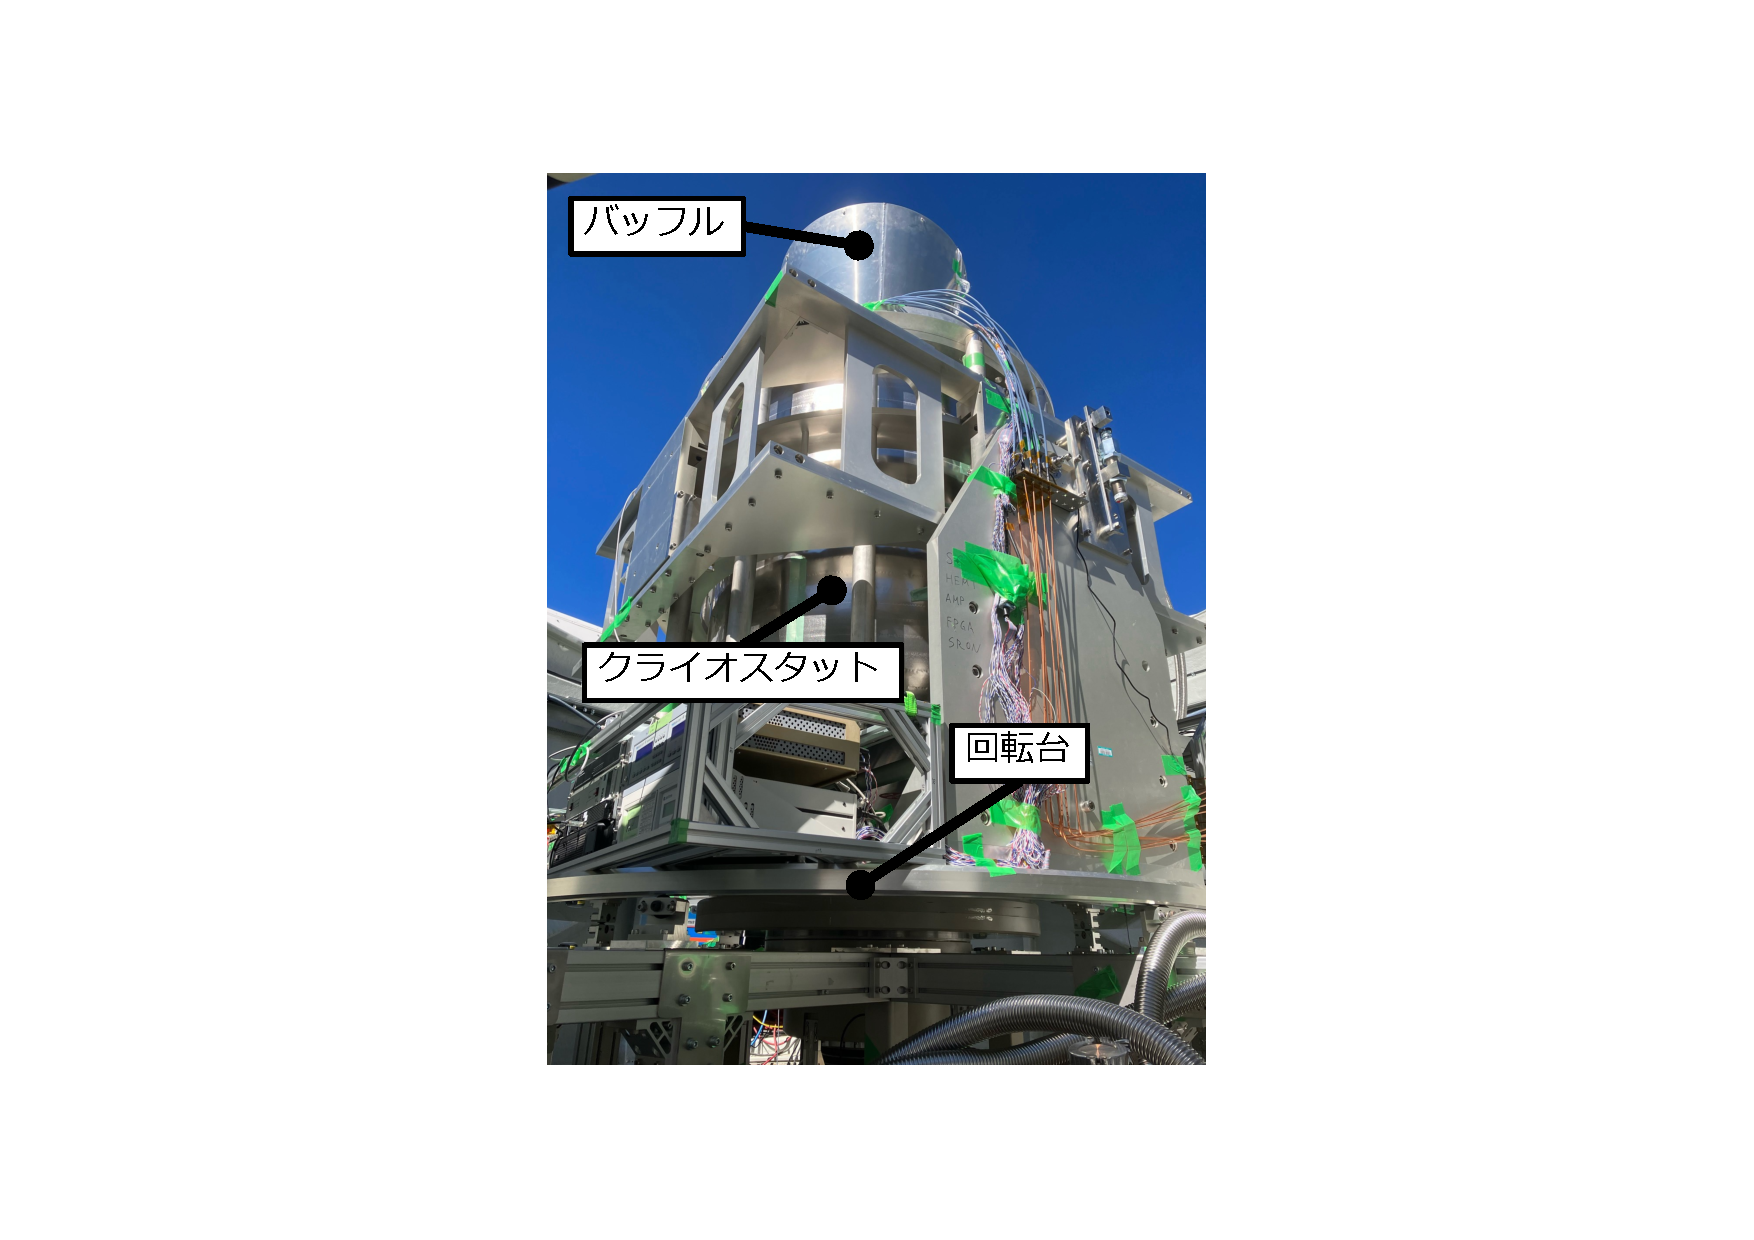
\includegraphics[width=0.5\columnwidth]{3_GB/figs/GB_overview2.pdf}
  \caption{GroundBIRD望遠鏡の外観。望遠鏡クライオスタットが方位角回転台の上に設置されており、回転台とともに最大で20RPM(1分間で20回転)の速度で回転する。}
  \label{GB_overview}
\end{figure}
\section{実験概要}

\subsection{GroundBIRD望遠鏡とスキャン戦略}
GroundBIRD望遠鏡はスペイン領カナリア諸島の1つであるテネリフェ島のテイデ観測所(高度2,400m)に位置する地上CMB望遠鏡である。地上からの観測において最も邪魔なのが大気からの放射であるが、テイデ観測所は大気中の積算水蒸気量(Precipitable Water Vapor、以下PWVと略す)がおよそ3.5mm\cite{PWV}と、観測に適した場所である。

GroundBIRDはスキャン戦略に大きな特徴を持つ。地上からの観測では大気放射に由来するノイズが本来見たいCMBに混入する。大気放射は無偏光であるが、観測装置の不完全性などで誤って偽偏光として観測されるおそれがある。特に、大気は刻一刻と揺らいでいるため、観測する空の領域ごとで観測される大気のノイズも揺らぎ、偽偏光を検出する影響は無視できなくなる。その影響を回避するためには大気揺らぎを抑制する変調が必要になる。GroundBIRDでは、望遠鏡を最大で20RPM(3秒で1回転)させる独自のスキャン戦略をとることで大気揺らぎを抑制したCMB観測を実現する。加えて望遠鏡の仰角を$70^{\circ}$に固定し、方位角方向に高速スキャンさせることで、全天の広い領域を観測することができる。望遠鏡の連続回転と地球の自転を組み合わせることで全天の約45$\%$を観測することができる(図\ref{scan_strategy})。

\begin{figure}[htbp]
  \centering
  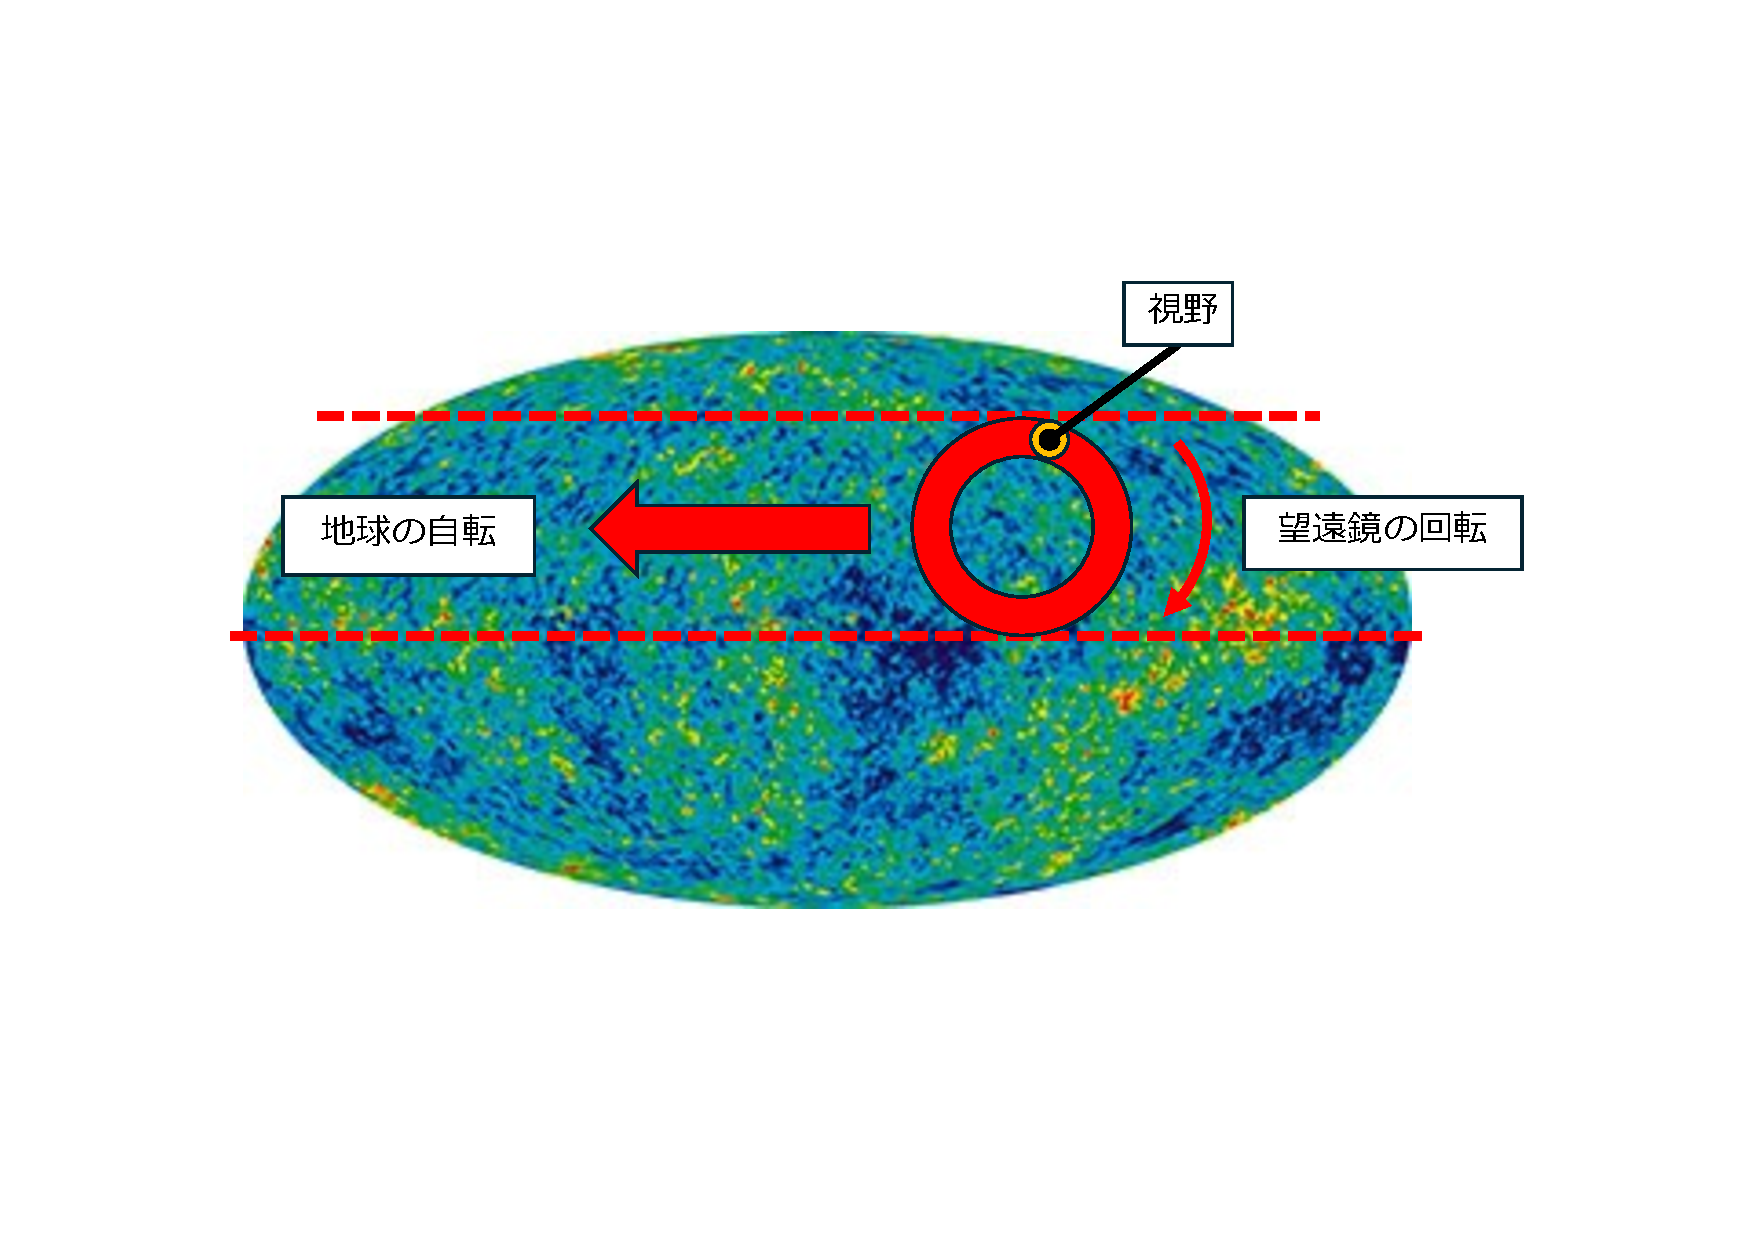
\includegraphics[width=0.8\columnwidth]{3_GB/figs/scan_strategy.pdf}
  \caption{GroundBIRDのスキャン戦略。GroundBIRDは視野$\pm 11^{\circ}$で観測する。望遠鏡の回転と地球の自転を組み合わせることで1日で全天の約半分をカバーできる。}
  \label{scan_strategy}
\end{figure}

次に、GroundBIRDの内部構造の概略を図\ref{GB_inside}に示す。光学系は放物面の主鏡と双曲面の副鏡から成り、CMBがバッフルから入り、光学系で2回反射させた後に、焦点面検出器ステージに入る。クライオスタット内は真空かつ低温になっており、外側のチャンバー部(300K)、40Kシールド、4Kシールドの3層から構成されている。4Kシールドの冷却にはパルスチューブ冷凍機を使用している。GroundBIRDでは超伝導検出器``MKID(Microwave Kinetic Inductance Detector)''を採用しているため、焦点面の温度は極低温に保つ必要がある。焦点面の冷却にはHeソープション冷凍機を使用し、温度を280mK付近に保持している。

\begin{figure}[htbp]
  \centering
  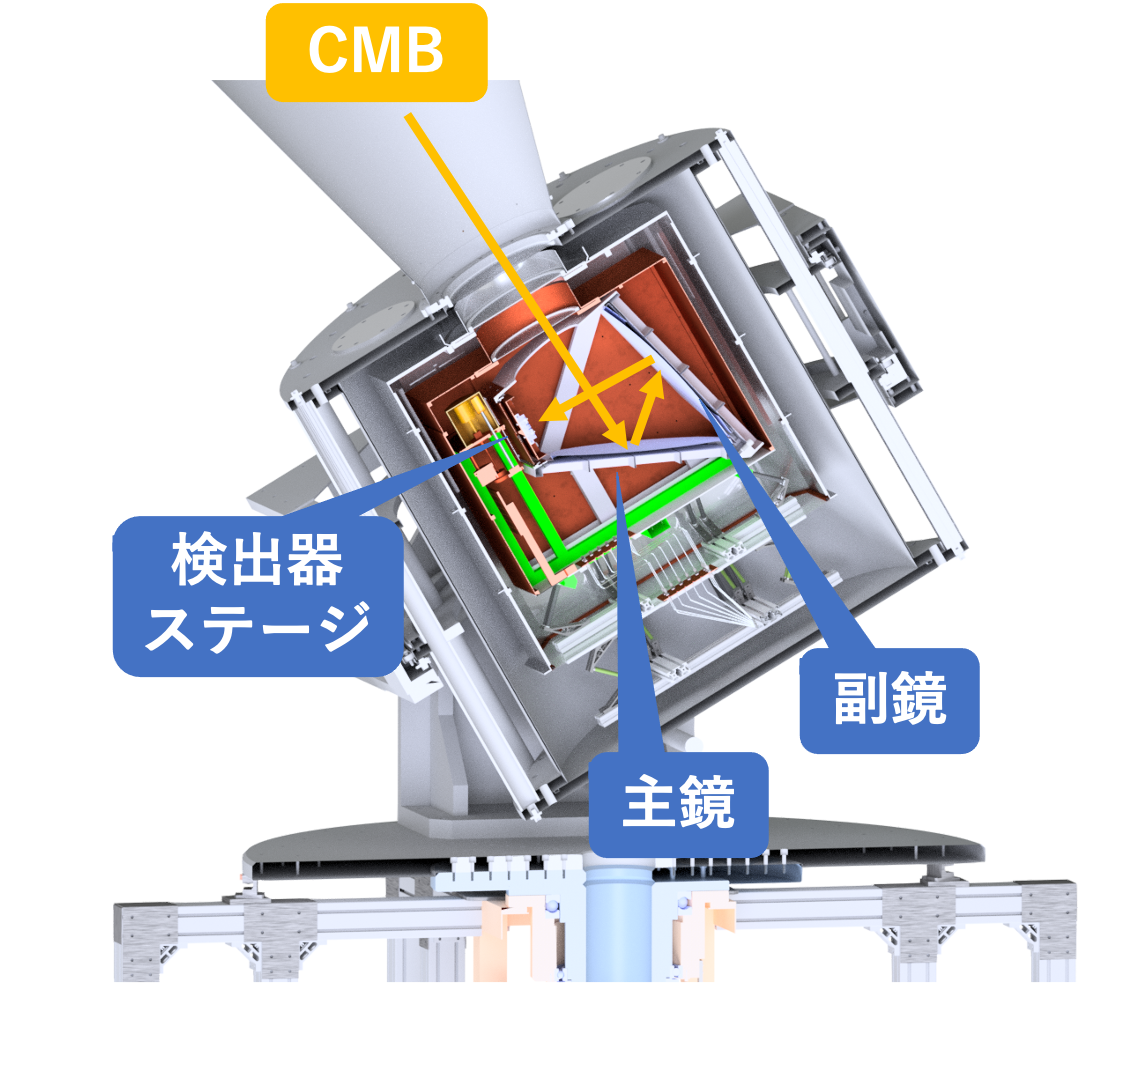
\includegraphics[width=0.6\columnwidth]{3_GB/figs/gb_int.png}
  \caption{GroundBIRD内部の概略図。バッフルを通ってCMBが望遠鏡内に入り、主鏡と副鏡で反射されて検出器ステージに入る。}
  \label{GB_inside}
\end{figure}

\subsection{超伝導検出器MKID}
GroundBIRDでは高速スキャンのもとで角度分解能を失わないようにサンプリングレートを1kHzにしている。そのため、検出器の応答時間が$< \mathcal{O}$(1)msであることが要求される。MKIDの典型的な応答時間は$< \mathcal{O}$(1)msであり\cite{MKID_res}、この要求を満たしている。CMB観測実験では他にも検出器として``TES(Transition Edge Sensor)''ボロメータを使うこともあるが、GroundBIRDでは時間応答性の面からMKIDを採用している。

MKIDの動作原理の概要を説明する。MKIDは超伝導共振回路を応用した高感度な光検出器である。入射する光子のエネルギーに応じて変化する回路内のインダクタンスを、数GHzで読み出す。MKIDの電子顕微鏡写真\cite{MKID_pic}と、等価回路を図\ref{mkid_pic}に示す。MKIDは読み出し線、超伝導体からなる共振器回路、アンテナからなっている。アンテナから電磁波が入射すると超伝導共振器の状態が変化し、そのインピーダンスの変化を読み出すことで入射エネルギーを測定する。具体的には、検出器の温度上昇やエネルギーが$h\nu > 2\Delta$($\Delta$は超伝導ギャップエネルギー)の光子との反応で、超伝導共振器内のクーパー対(結合した電子対)が壊れる。対になっていた電子はエネルギーギャップより上の準位へと押し上げられる(図\ref{cooper})。この過程で生成される電子を準粒子という。準粒子によって共振器内の超伝導状態が変化し、可変インダクタンスの値が変化する。また、1つの読み出し線に複数の共振器が容量性カップリング(Capacitive coupling; Cカップリング)しており、1対の読み出し配線を使って$\mathcal{O}$(1000)個のMKIDを同時に読み出すことができる。

\begin{figure}[h]
  \begin{tabular}{cc}
    %---- 最初の図 ---------------------------
    \begin{minipage}[t]{0.45\hsize}
      \centering
      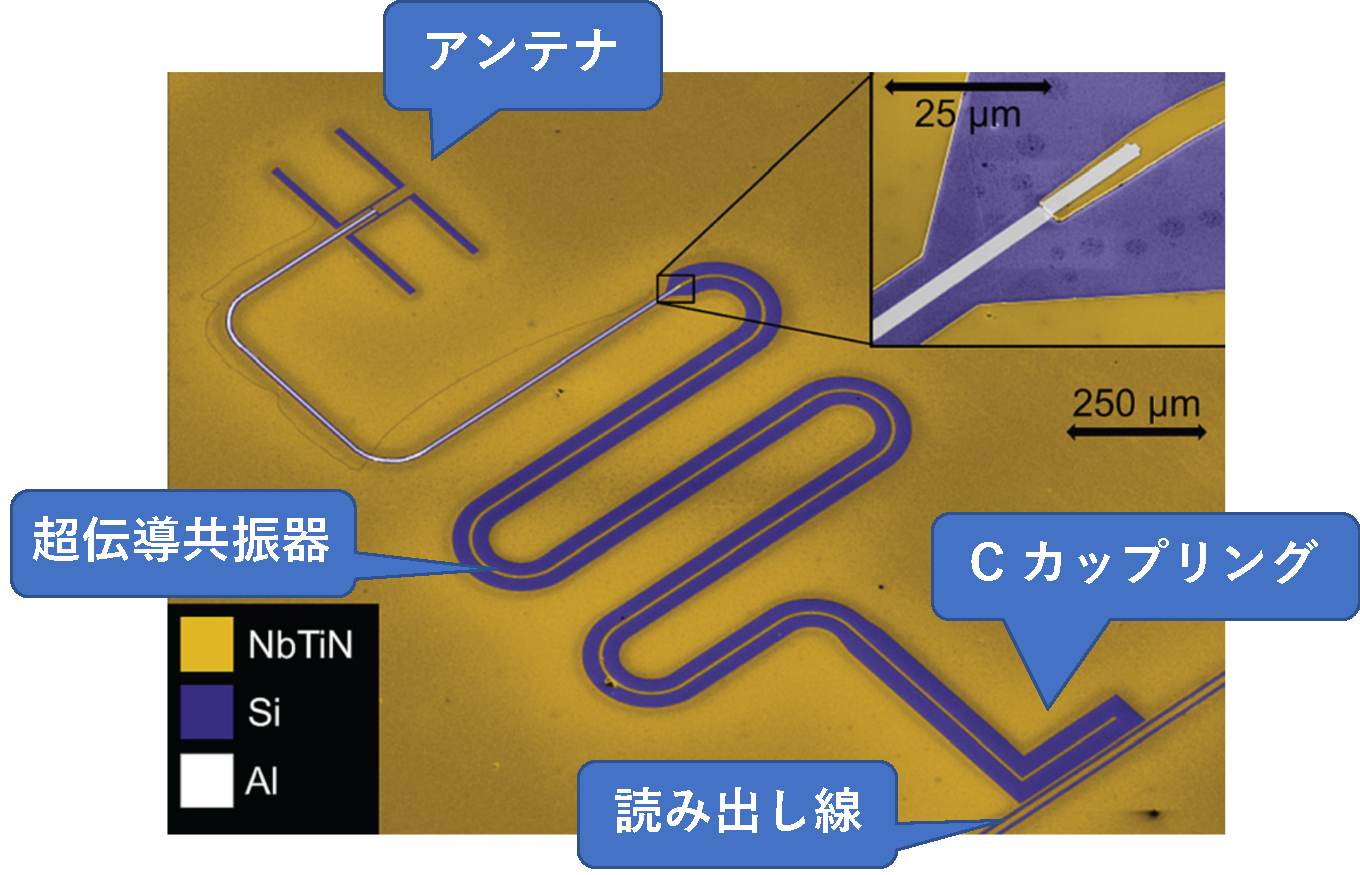
\includegraphics[keepaspectratio, scale=0.3]{3_GB/figs/mkid_pic.pdf}
      \subcaption{MKIDの電子顕微鏡写真\cite{MKID_pic}。読み出し線、超伝導共振器、アンテナからなる。}
    \end{minipage}
    %---- 2番目の図 --------------------------
    \begin{minipage}[t]{0.45\hsize}
      \centering
      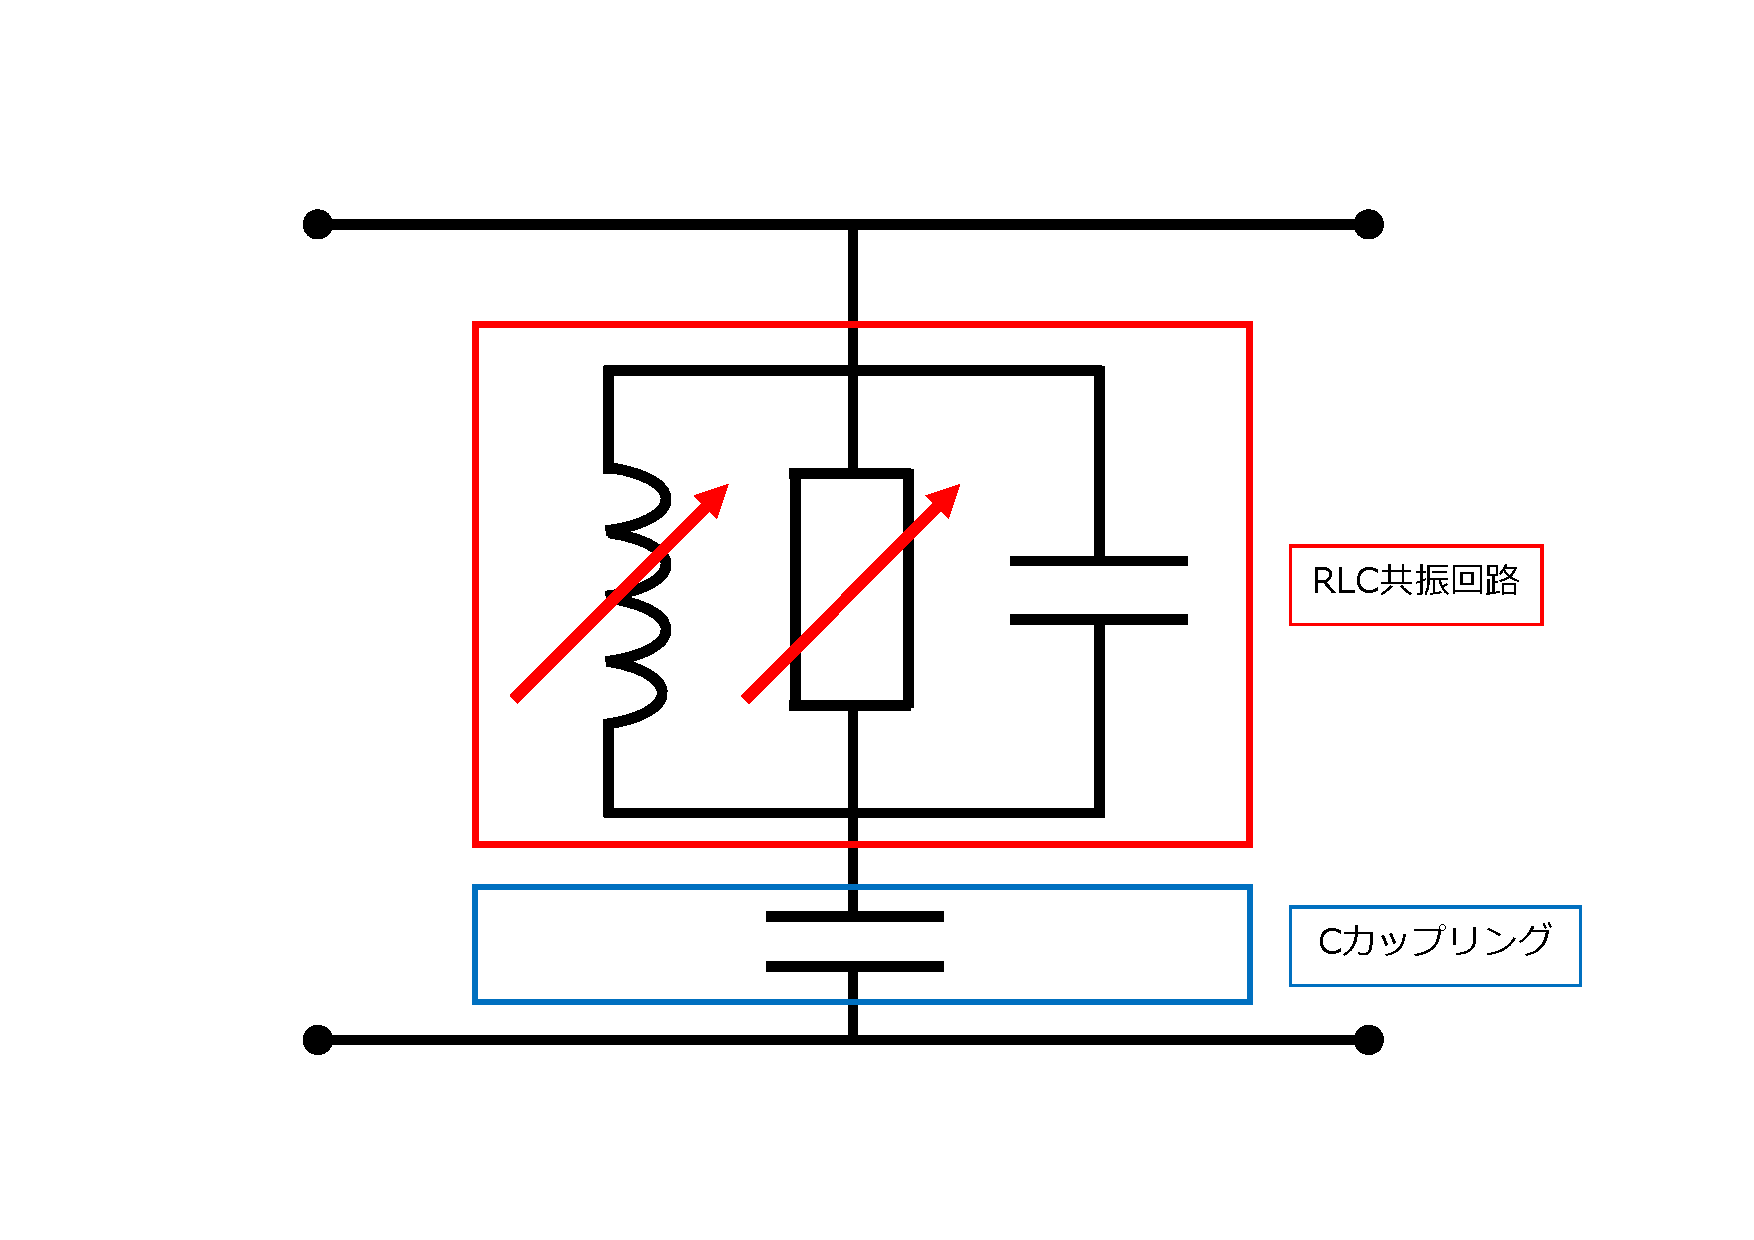
\includegraphics[keepaspectratio, scale=0.3]{3_GB/figs/mkid_circ.pdf}
      \subcaption{MKIDの等価回路。可変インダクタンスと可変抵抗をもつRLC共振回路になっている。}
    \end{minipage}
    %---- 図はここまで ----------------------
  \end{tabular}
  \caption{超伝導検出器MKID}
  \label{mkid_pic}
\end{figure}

\begin{figure}[htbp]
  \centering
  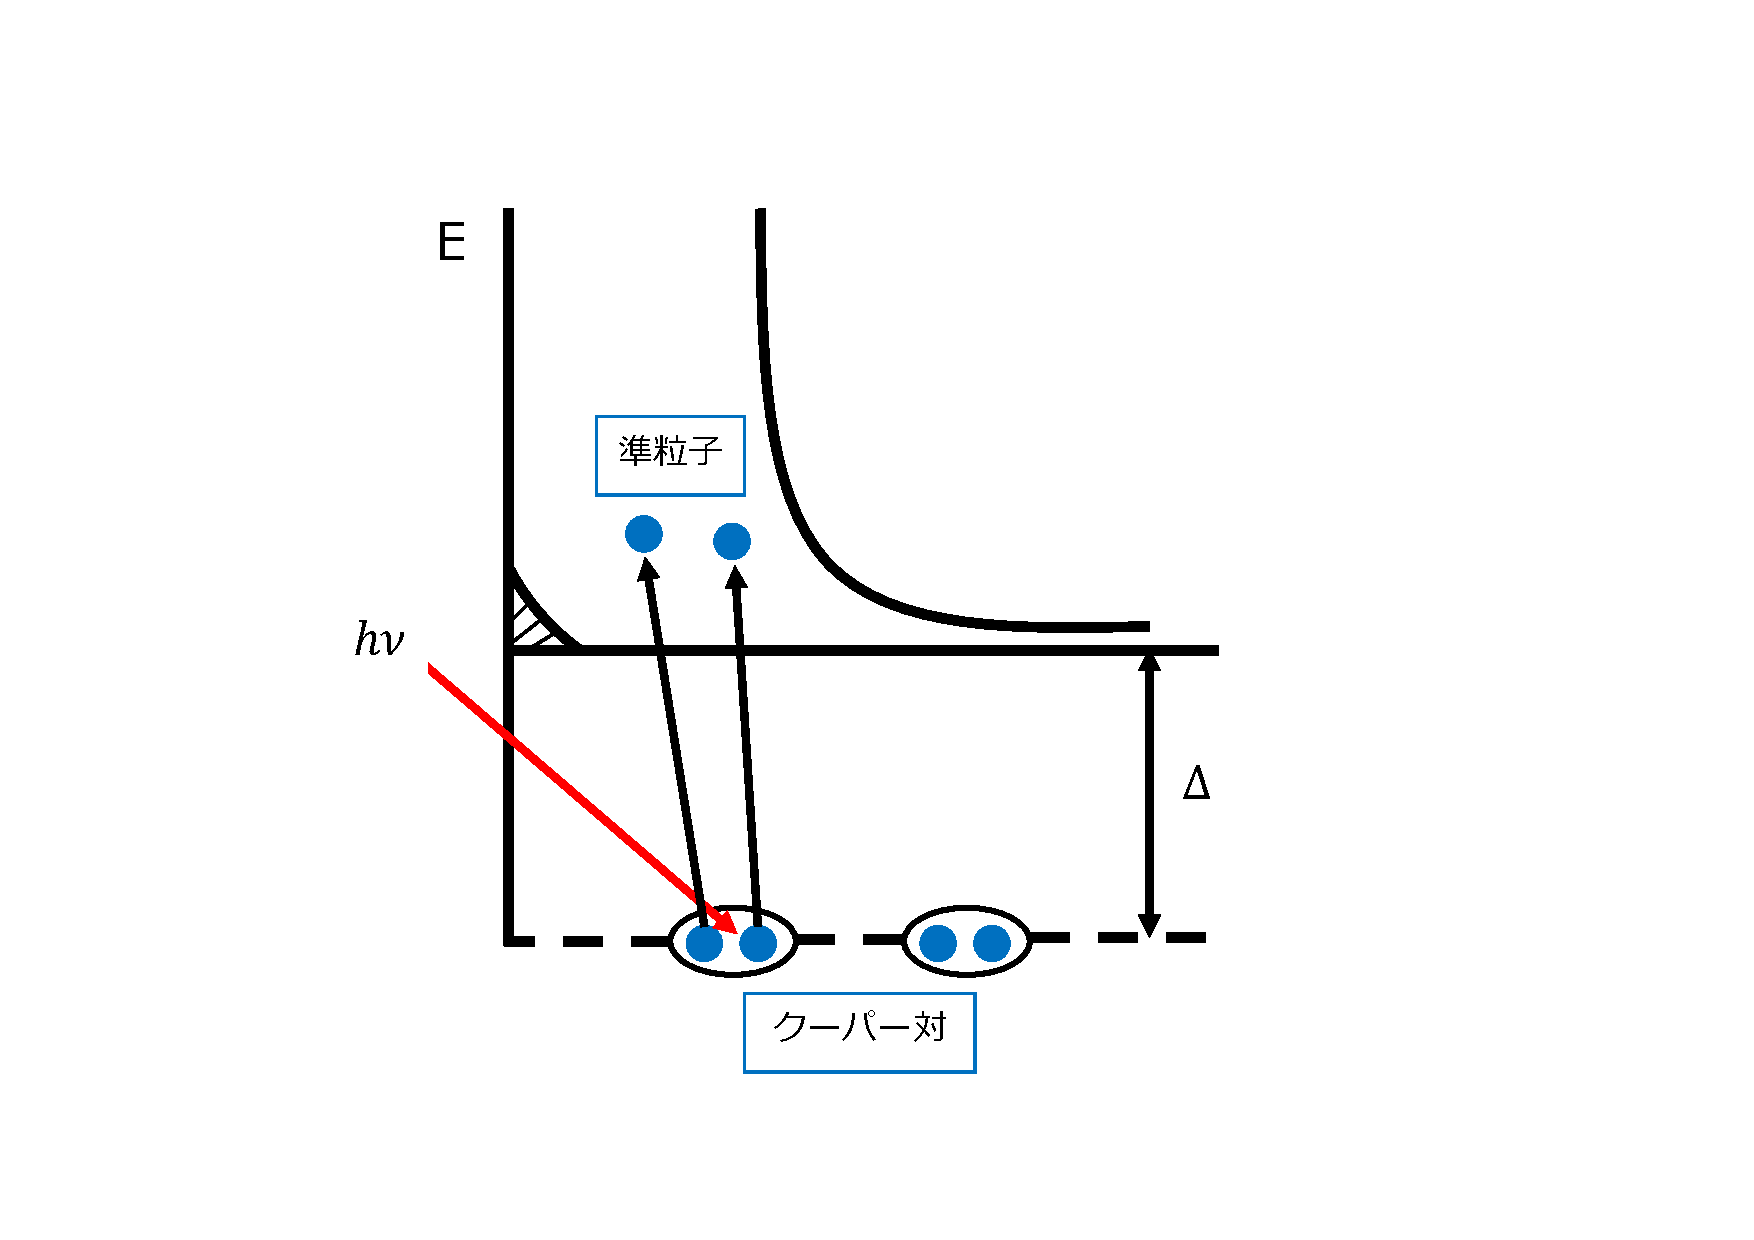
\includegraphics[width=0.6\columnwidth]{3_GB/figs/cooper.pdf}
  \caption{入射光子による準粒子生成の模式図。縦軸は電子のエネルギーを表す。$h\nu > 2\Delta$のエネルギーを持つ光が超伝導共振器に入射すると、クーパー対が壊されてエネルギー準位が押し上げられ、準粒子になる。}
  \label{cooper}
\end{figure}

\subsection{物理ターゲット}
GroundBIRDが探る物理ターゲットは\ref{E_and_tau}で見た光学的厚み$\tau$の地上からの再測定である。光学的厚み$\tau$の測定は今までにWMAPやPlanckといった衛星実験によって測定がされてきた。図\ref{tau_planck}に測定された$\tau$の値の変遷を示す。誤差が小さくなってきており、最新の測定結果ではその誤差は$\sim 10\%$である。しかし、平均値は系統的に下がっている傾向にあり、独立した測定によってこの結果の妥当性を評価する必要がある。そのため、地上実験(例えばCLASS\cite{CLASS}やQUIJOTE\cite{QUIJOTE}など)からの$\tau$の精密測定が始まっている。

\begin{figure}[htbp]
  \centering
  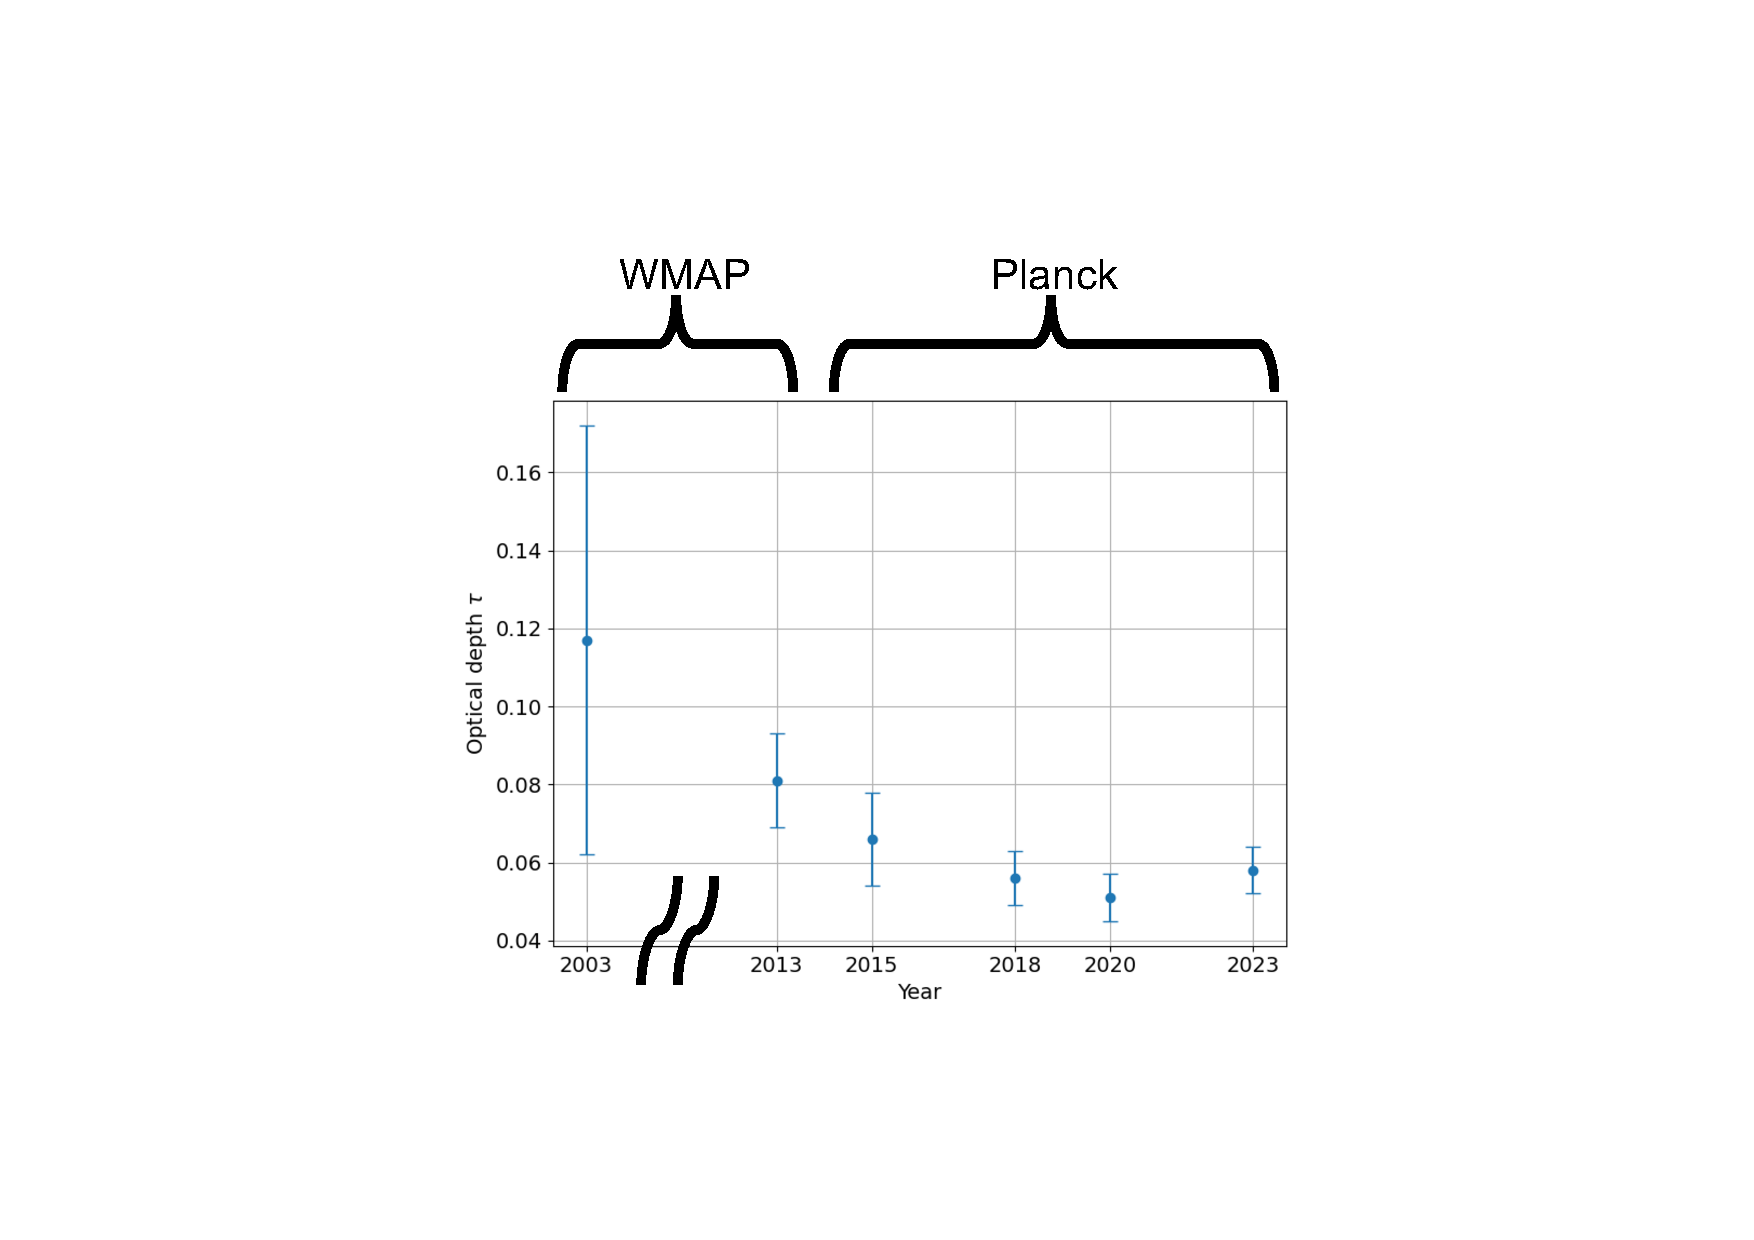
\includegraphics[width=0.8\columnwidth]{3_GB/figs/tau_planck_wmap_cut.pdf}
  \caption{WMAPとPlanckによって測定された光学的厚み$\tau$の値\cite{tau_measure}。最新では誤差は$\sim 10\%$である。}
  \label{tau_planck}
\end{figure}

\section{現在の観測状況}

\subsection{検出器のフルアレイインストール}

\subsection{リモート観測システム}

\section{本論文の構成}
